\section{热力学第一定律}
\begin{question}{题目4.2.1}
    $1 \,\si{mol}$ 气体做准静态等温膨胀,由初体积$V_\mathrm{i,m}$ 变成终体积 $V_\mathrm{f,m}$,试计算这过程中系统对外界所做的功. 物态方程分别为
    \begin{enumerate}
        \item[(1)] $p(V_\mathrm{m} - b) = RT$ ($R$,$b$是常量)
        \item[(2)] $pV_\mathrm{m} = RT\left(1-\dfrac{B}{V_\mathrm{m}}\right)$ ($R$为常量,$B = f(T)$)
    \end{enumerate}
\end{question}

\begin{solution}
    (1)根据题目所给的物态方程,得到压强 $p$ 的表达式为
    $$
        p = \frac{RT}{V_\mathrm{m} - b}
    $$
    准静态等温膨胀过程中所做的功为
    $$
        W  = \int_{V_\mathrm{i,m}}^{V_\mathrm{f,m}} p \,\mathrm{d}V_\mathrm{m}
        = \int_{V_\mathrm{i,m}}^{V_\mathrm{f,m}} \frac{RT}{V_\mathrm{m} - b} \,\mathrm{d}V_\mathrm{m}
        = RT\ln\frac{V_\mathrm{f,m} - b}{V_\mathrm{i,m} - b}
    $$
    (2)根据题目所给的物态方程,得到压强 $p$ 的表达式为
    $$
        p = RT\left(\frac{1}{V_\mathrm{m}} - \frac{B}{V_\mathrm{m}^2}\right)
    $$
    准静态等温膨胀过程中所做的功为
    $$
        W  = \int_{V_\mathrm{i,m}}^{V_\mathrm{f,m}} p \,\mathrm{d}V_\mathrm{m}
        = RT \int_{V_\mathrm{i,m}}^{V_\mathrm{f,m}} \left(\frac{1}{V_\mathrm{m}} - \frac{B}{V_\mathrm{m}^2} \right) \,\mathrm{d}V_\mathrm{m}
        = RT\ln\frac{V_\mathrm{f,m}}{V_\mathrm{i,m}} + \frac{BRT}{V_\mathrm{f,m}} - \frac{BRT}{V_\mathrm{i,m}}
    $$
\end{solution}

\begin{question}{题目4.4.2}
    已知范德瓦耳斯气体物态方程为
    $$
        \left(p+\frac{a}{V_\mathrm{m}^2}\right)\left(V_\mathrm{m}-b\right) = RT,
    $$
    其内能为
    $$
        U_\mathrm{m} = cT - \frac{a}{V_\mathrm{m}^2} + d,
    $$
    其中 $a$,$b$,$c$,$d$ 均为常量.试求:
    \begin{enumerate}
        \item[(1)] 该气体从 $V_1$ 等温膨胀到 $V_2$ 时系统对外界所做的功;
        \item[(2)] 该气体在定体下升高 $\Delta T$ 温度所吸收的热量.
    \end{enumerate}
\end{question}
\begin{solution}
    (1)改写方程得到 $p$ 的表达式,并代入做功表达式
    $$
        W'  = \int_{V_\mathrm{1,m}}^{V_\mathrm{2,m}} p \,\mathrm{d}V_\mathrm{m}
        = \int_{V_\mathrm{1,m}}^{V_\mathrm{2,m}} \left(\frac{RT}{V_\mathrm{m}-b} - \frac{a}{V_\mathrm{m}^2} \right) \,\mathrm{d}V_\mathrm{m}
        = RT\ln\frac{V_\mathrm{2,m} - b}{V_\mathrm{1,m}-b} + \frac{a}{V_\mathrm{2,m}} - \frac{a}{V_\mathrm{1,m}}.
    $$
    (2)定体情况下气体不向外做功,所以吸收的热量会全部转化为气体内能
    $$
        \Delta{Q} = \Delta{U} = c( T + \Delta T ) - \frac{a}{V_\mathrm{m}^2} + d -\left(cT - \frac{a}{V_\mathrm{m}^2} + d\right) = c \cdot \Delta{T}.
    $$
\end{solution}

\begin{question}{题目4.4.4}
    实验数据表明,在 $0.1 \,\si{MPa}$,$300-1200 \,\si{K}$ 范围内铜的摩尔定压热容为 $C_{p,\mathrm{m}} = a + bT$,其中 $a = 2.3 \times 10^{4} \,\si{J \cdot mol^{-1} \cdot K^{-1}}$,$b = 5.92 \,\si{J \cdot mol^{-1} \cdot K}$. 试计算在 $0.1 \,\si{MPa}$ 下,温度从 $300\,\si{K}$ 增到 $1200\,\si{K}$ 时铜的摩尔焓的改变.
\end{question}
\begin{solution}
    由于温度在 $300 \,\si{K}$ 增到 $1200\,\si{K}$ 的过程中铜的压强不变,因而它吸收的热量等于焓的改变
    $$
        H_\mathrm{m} = \Delta{Q}_\mathrm{m} = \int_{T_1}^{T_2} C_{p,\mathrm{m}} \,\mathrm{d}T = \int_{T_1}^{T_2} (a+bT) \,\mathrm{d}T = 2.47 \times 10^7 \,\si{ J \cdot mol^{-1} }
    $$
\end{solution}

\begin{question}{题目4.4.6}
    设 $1 \,\si{mol}$ 固体的物态方程可写为
    $$
        V_\mathrm{m} = V_\mathrm{0,m} + aT + bp,
    $$
    摩尔内能可表示为
    $$
        U_\mathrm{m} = cT - apT,
    $$
    其中 $a,b,c,V_\mathrm{0,m}$均是常量,试求:
    \begin{enumerate}
        \item[(1)] 摩尔焓的表达式
        \item[(2)] 摩尔热容 $C_{p,\mathrm{m}}$ 和 $C_{V,\mathrm{m}}$
    \end{enumerate}
\end{question}
\begin{solution}
    (1)根据焓的定义 $H = U + pV$ 我们有
    $$
        H_\mathrm{m} = U_\mathrm{m} + pV_\mathrm{m} = cT + pV_{0,\mathrm{m}} + bp^2.
    $$
    (2)根据摩尔热容的定义 $C_{p,\mathrm{m}} = \left( \dfrac{\partial H_\mathrm{m}}{\partial T}\right)_p$ 我们有
    $$
        C_{p,\mathrm{m}} = \left( \frac{\partial H_\mathrm{m}}{\partial T}\right)_p = c
    $$
    对于 $1 \,\si{mol}$ 固体,有
    $$
        V_\mathrm{m} = V_{0,\mathrm{m}} + aT + bp
        \implies
        p = \frac{V_\mathrm{m} - V_\mathrm{0,m} - aT}{b}
    $$
    则内能可以表示为
    $$
        U_\mathrm{m}
        = cT - apT
        = cT - a\frac{V_\mathrm{m} - V_\mathrm{0,m} - aT}{b}T
    $$
    于是根据摩尔热容的定义 $C_{V,\mathrm{m}} = \left( \dfrac{\partial U_\mathrm{m}}{\partial T}\right)_V$ 我们有
    $$
        C_{V,\mathrm{m}}
        = \left(\frac{\partial U_\mathrm{m}}{\partial T}\right)_V
        = c - \frac{a}{b}V_\mathrm{m} + \frac{aV_{0,\mathrm{m}}}{b} + \frac{2a^2T}{b}.
    $$
\end{solution}

\begin{question}{题目4.5.1}
    有一除底部外都是绝热的气筒,被一位置固定的导热板隔成相等的两部分 $A$ 和 $B$,其中各盛有 $1 \,\si{mol}$ 的理想气体氮. 今将 $334.4\,\si{J}$ 的热量缓慢地由底部供给气体,设活塞上的压强始终保持为 $0. 101 \,\si{MPa}$,求 $A$ 部和 $B$ 部温度的改变以及各吸收的热量(导热板的热容可以忽略).若将位置固定的导热板换成可以自由滑动的绝热隔板,重复上述讨论.
\end{question}
\begin{solution}
    (1) $A$部经历等体过程
    $$
        \Delta Q_A = \Delta U_\mathrm{m} = C_{V,\mathrm{m}}\Delta{T_A}
    $$
    $B$部经历等压过程
    $$
        \Delta Q_B = \Delta H_\mathrm{m} = C_{p,\mathrm{m}}\Delta{T_B}
    $$
    由于隔板是导热的,所以稳态时 $T_A = T_B$ ,也即 $\Delta T_A = \Delta T_B = \Delta T$,而体系吸收的总热量为 $\Delta Q = 334.4 \,\si{J}$
    $$
        \Delta Q = \Delta{Q_A} + \Delta{Q_B}
        = (C_{V,\mathrm{m}} +C_{p,\mathrm{m}})\Delta{T}
        = 6R \cdot \Delta{T}
        =  334.4 \,\si{J}
    $$
    进一步解得 $\Delta T$,$\Delta Q_A$ 和 $\Delta Q_B$
    $$
        \Delta T = 6.70 \,\si{K}
    $$
    $$
        \Delta Q_A = C_{V,\mathrm{m}}\Delta{T} = \frac{5}{2}R\Delta{T} = 139.27 \,\si{J}
    $$
    $$
        \Delta Q_B = C_{p,\mathrm{m}}\Delta{T} = \frac{7}{2}R\Delta{T} = 194.97 \,\si{J}
    $$
    (2) 若隔板是可以自由滑动的而且是绝热的,则 $A$ 部吸收热量后按照等压过程变化; $B$ 部不吸收热量,也不做功(因为它通过活塞和外界相连接,它的压强始终和外界相等),按照热力学第一定律,其内能不变,状态也不变. $A$ 部吸收的热量全部用于 $A$ 部内能的增加和它对外做的等压功.
    $$
        \Delta Q_A = C_{p,\mathrm{m}} \Delta{T}
        = \frac{7}{2}R\Delta{T} = 334.4 \,\si{K}
    $$
    $$
        \Delta T = \frac{\Delta Q}{\frac{7}{2}R}
        = 11.49 \,\si{K}.
    $$
    $B$ 部与活塞连接,压强恒为$1 \,\si{atm}$,且因为隔板是隔热的,所以它不吸收热量,也不对外做功.
\end{solution}

\begin{question}{题目4.5.2}
    分别通过下列过程把标准状态下的 $0.14 \,\si{kg}$ 氮气压缩为原体积的一半:
    \begin{enumerate}
        \item[(1)] 等温过程;
        \item[(2)] 绝热过程;
        \item[(3)] 等压过程;
    \end{enumerate}
    试分别求出在这些过程中气体内能的改变,传递的热量和外界对气体所做的功,设氮气可看做理想气体,且 $C_{V,\mathrm{m}} = \dfrac{5}{2}R$.
\end{question}
\begin{solution}
    (1)等温过程中 $\Delta{U} = 0$,外界对气体做的功为
    $$
        W = - \nu RT \ln \frac{V_2}{V_1} = 7862 \,\si{J}
    $$
    气体对外放热
    $$
        \Delta{Q} = 7862 \,\si{J}
    $$
    (2)绝热过程中 $\Delta{Q} = 0$,根据绝热过程方程,有
    $$
        T_2 = \left(\frac{V_1}{V_2}\right)^{\gamma - 1} T_1
    $$
    外界对气体做的功为
    $$
        W  = \Delta{U} = \nu C_{V,\mathrm{m}} (T_2 - T_1)
        = \nu C_{V,\mathrm{m}}T_1\left[ \left(\frac{V_1}{V_2}\right)^{\gamma - 1} -1 \right]
        = 9061 \,\si{J}
    $$
    (3)等压过程有 $\frac{T_2}{V_2} = \frac{T_1}{V_1}$,气体内能的变化为
    $$
        \Delta{U}
        = \nu C_{V,\mathrm{m}} (T_2 - T_1)
        = \nu C_{V,\mathrm{m}} T_1 \left( \frac{V_1}{V_2} - 1 \right)
        = -1.41 \times 10^4 \,\si{J}
    $$
    气体放热为
    $$
        \Delta{Q} = \nu C_{p,\mathrm{m}} (T_2 - T_1) = -1.97 \times 10^4 \,\si{J}
    $$
    外界对气体做功
    $$
        W = \Delta{U} - \Delta{Q} = 5.6 \times 10^3 \,\si{J}
    $$
\end{solution}

\begin{question}{题目4.5.3}
    在标准状态下的 $0.016 \,\si{kg}$ 的氧气,分别经过下列过程从外界吸收了 $334.4 \,\si{J}$ 的热量:
    \begin{enumerate}
        \item[(1)] 若为等温过程,求终态体积;
        \item[(2)] 若为等容过程,求终态压强;
        \item[(3)] 若为等压过程,求气体内能的变化;
    \end{enumerate}
    设氧气可看做理想气体,且 $C_{V, \mathrm{m}} = \dfrac{5}{2}R$
\end{question}
\begin{solution}
    初始状态下氧气的各项参量:
    $$
        \nu = \frac{m}{M} = 0.5 \,\si{mol}
        \quad \quad
        p_1 = 1.01 \times 10^5 \,\si{Pa}
        \quad \quad
        T_1 = 273.15 \,\si{K}
        \quad \quad
        V_1 = 11.2 \,\si{L}
    $$
    (1)气体吸热后等温膨胀,内能不变,吸收的热量全部对外做功
    $$
        Q = W  = \int_{V_1}^{V_2} p_1 \,\mathrm{d}V
        = \int_{V_1}^{V_2} \frac{\nu RT_1}{V} \,\mathrm{d}V
        = \nu RT_1 \ln\frac{V_2}{V_1}
    $$
    解得
    $$
        V_2 = V_1 \exp \left(\frac{Q}{\nu RT_1}\right) = 15.04 \,\si{L}
    $$
    (2)气体吸热后等体升温,根据物态方程 $pV = \nu RT$,有
    $$
        \frac{p_1}{T_1} = \frac{p_2}{T_2}
    $$
    同时,等体过程中气体吸收的热量会全部转化为内能
    $$
        Q = U_\mathrm{m} = \nu C_{V,\mathrm{m}}(T_2 - T_1)
        = \frac{5\nu R}{2} \left(\frac{p_2}{p_1} - 1\right)T_1
        = 334.4 \,\si{J}
    $$
    解得 $p_2$
    $$
        p_2 = \left(\frac{2Q}{5 \nu RT_1}+1 \right) p_1 = 1.13 \times 10^5 \,\si{Pa}
    $$
    (3)气体吸热后等压膨胀,吸热过程可以表示为
    $$
        Q = \nu C_{p,\mathrm{m}} (T_2 -T_1) = 334.4 \,\si{J}
    $$
    而内能变化可以表示为
    $$
        U_\mathrm{m} = \nu C_{V,\mathrm{m}}(T_2 - T_1)
        = \frac{Q}{C_{p,\mathrm{m}}} C_{V,\mathrm{m}}
        = 238.86 \,\si{J}
    $$
\end{solution}

\begin{question}{题目4.5.5}
    室温下一定量理想气体氧的体积为 $2.3 \,\si{L}$,压强为 $0.1 \,\si{MPa}$,经过某一多方过程后体积变为 $4.1 \,\si{L}$,压强为 $0.05 \,\si{MPa}$.设氧气 $C_{V, \mathrm{m}} = \dfrac{5}{2}R$,试求:
    \begin{enumerate}
        \item[(1)] 多方指数 $n$;
        \item[(2)] 内能的变化;
        \item[(3)] 吸收的热量;
        \item[(4)] 氧膨胀时对外界所做的功;
    \end{enumerate}
\end{question}
\begin{solution}
    (1)多方过程的方程为 $pV^n = C$,即
    $$
        p_1V_1^n =p_2V_2^n
    $$
    移项整理并取对数,解得
    $$
        n = \frac{
            \ln \left(\dfrac{p_1}{p_2}\right)
        }{
            \ln \left(\dfrac{V_2}{V_1}\right)
        }
        = 1.20
    $$
    (2)根据物态方程 $pV = \nu RT$可以得到
    $$
        p_1V_1 = \nu RT_1
        \quad \quad
        p_2V_2 = \nu RT_2
    $$
    而理想气体的内能变化可以表示为
    $$
        \Delta U
        = \nu C_{V,\mathrm{m}}(T_2 -T_1)
        = \nu \frac{5R}{2} \left(\frac{p_2V_2}{\nu R} - \frac{p_1V_1}{\nu R}\right)
        = -62.5 \,\si{J}
    $$
    (3)多方过程的热容为
    $$
        C_{n,m} = C_{V,m} - \frac{R}{n-1}
    $$
    多方过程中吸收的热量为
    $$
        Q = \nu C_{n,m} (T_2 - T_1)
        = \nu \left(\frac{5R}{2} - \frac{R}{1.20 - 1}\right) \left(\frac{p_2V_2}{\nu R} - \frac{p_1V_1}{\nu R}\right)
        = 62.5 \,\si{J}
    $$
    (4) 根据热力学第一定律,系统内能变化为
    $$
        \Delta U = Q + W
    $$
    则系统对外做功 $W'$ 可以表示为
    $$
        W' = -W = Q - \Delta{U} = 62.5 - (-62.5) = 125 \,\si{J}
    $$
\end{solution}

\begin{question}{题目4.5.16}
    有 $28 \,\si{g}$ 氮气经摩尔热容 $C_{1,\mathrm{m}} =2R$ 的平衡过程,从标准状态开始体积膨胀了 $4$ 倍. 试问:
    \begin{enumerate}
        \item[(1)] 该过程满足什么样的方程?
        \item[(2)] 在该过程中对外做了多少功,改变了多少内能,吸(或放)了多少热量?
    \end{enumerate}
\end{question}
\begin{solution}
    (1)根据热力学第一定律,可知此过程中氮气吸收的热量会转化为自身内能和对外做功
    $$
        C_{V,\mathrm{m}} \,\mathrm{d}T = C_{1,\mathrm{m}} \,\mathrm{d}T - p \,\mathrm{d}V
    $$
    其中 28g 氮气的 $C_{V,\mathrm{m}} = \dfrac{5R}{2}$,$C_{1,\mathrm{m}} = 2R$, $\nu = 1 \,\si{mol}$
    $$
        \frac{R}{2} \ \mathrm{d}T = -p \ \mathrm{d}V
    $$
    根据物态方程 $pV = \nu RT$ 消去 $T$,并分离变量
    $$
        \begin{aligned}
            \frac{R}{2} \,\mathrm{d}\left(\frac{pV}{R}\right)      & = -p \,\mathrm{d}V         \\
            \frac{1}{2} \left(p\,\mathrm{d}V + V\mathrm{d}p\right) & = -p \,\mathrm{d}V         \\
            \frac{\mathrm{d}p}{p}                                  & = -3 \frac{\mathrm{d}V}{V} \\
        \end{aligned}
    $$
    两边积分并整理
    $$
        \begin{aligned}
            \int\frac{\mathrm{d}p}{p} & = -3 \int\frac{\mathrm{d}V}{V} \\
            \ln{p} + C_1              & = -3\ln{V} + C_2               \\
            pV^3                      & = C
        \end{aligned}
    $$
    \paragraph{方法二}
    根据理想气体多方过程的热容公式,求出 $C_{n,\mathrm{m}}$
    $$
        C_{n,\mathrm{m}}
        = C_{V,\mathrm{m}} - \frac{R}{n-1}
        = C_{V,\mathrm{m}} \cdot \frac{\gamma-n}{1-n}
        = 3
    $$
    于是方程为
    $$
        pV^3 = C
    $$
    (2) $28 \,\si{g}$ 氮气在标准状态下时
    $$
        \nu = 1 \,\si{mol},
        \quad\quad
        p_0 = 1.01 \times 10^5 \,\si{Pa},
        \quad\quad
        V_0 = 22.4 \,\si{L},
        \quad\quad
        T_0 = 273.15\,\si{K}
    $$
    经历多方过程后,体积膨胀为初始状态的 $4$ 倍($V_2 = 4V_0 = 89.6 \,\si{L}$)压强变为 $p_2$
    $$
        p_2 = p_1 \left(\dfrac{V_1}{V_2}\right)^3
        = \frac{12625}{8} \,\si{Pa}
    $$
    温度变为
    $$
        T_2 = \dfrac{p_1V_1}{p_2V_2}T_1 = \frac{5463}{320} \,\si{K}
    $$
    氮气的内能改变量 $\Delta U$ 为
    $$
        \Delta U
        = \nu C_{V,\mathrm{m}} (T_2-T_1)
        %= 1 \times \frac{5R}{2} \times \left(\frac{5463}{320} - 273.15\right)
        = - 5324.63 \,\si{J}
    $$
    氮气吸收的热量 $\Delta Q$ 为
    $$
        \Delta Q
        = \nu  C_{1,\mathrm{m}} (T_2 - T_1)
        %= 1 \times 2R \times \left(\frac{5463}{320} - 273.15\right)
        = -4259.71 \,\si{J}
    $$
    系统对外做功 $W'$ 为
    $$
        W' = -W = \Delta Q - \Delta U =  1064.92 \,\si{J}
    $$
\end{solution}

\begin{question}{题目4.6.1}
    已知某种理想气体在 $p-V$ 图上的等温线与绝热线的斜率之比为 $0.714$,现 $1 \,\si{mol}$ 该种理想气体在 $p-T$ 图上经历如图所示的循环,试问:
    \begin{enumerate}
        \item [(1)] 该气体的 $C_{V,\mathrm{m}}$ 是多少?
        \item [(2)] 循环中所做的功是多少?
        \item [(3)] 循环效率是多少?
    \end{enumerate}
    \centering
    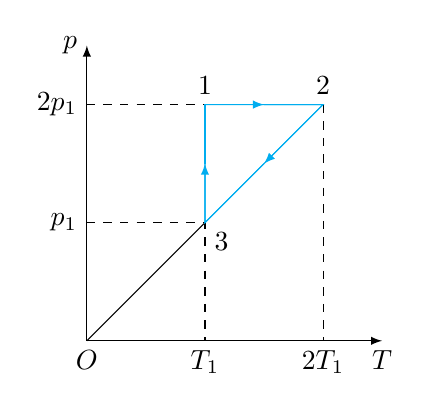
\begin{tikzpicture}[scale = 1.5, domain = 0:3]
        %画坐标轴
        \draw[-latex] (0,1) -- (0, 0) -- (2.5, 0) node[below] {$T$};
        \draw[-latex] (1,0) -- (0, 0) -- (0, 2.5) node[left ] {$p$};
        \node[below] at (0,0) {$O$};

        %画出虚线辅助线
        \draw (0, 0) -- (1, 1);
        \draw[dashed] (0, 1) -- (1, 1) -- (1, 0);
        \draw[dashed] (0, 2) -- (1, 2);
        \draw[dashed] (2, 2) -- (2, 0);

        %画出三个循环的箭头
        \draw[-latex, cyan] (1, 1.5) -- (1,2) -- (1.5, 2);
        \draw[-latex, cyan] (1.5, 2) -- (2,2) -- (1.5, 1.5);
        \draw[-latex, cyan] (1.5, 1.5) -- (1,1) -- (1, 1.5);
        \draw[cyan] (1, 1) -- (1, 2) -- (2, 2) -- (1, 1) -- cycle;

        %标注出各个点
        \node[left] at (0, 1) {$p_1$};
        \node[left] at (0, 2) {$2p_1$};
        \node[below] at (1, 0) {$T_1$};
        \node[below] at (2, 0) {$2T_1$};
        \node[above] at (1, 2) {$1$};
        \node[above] at (2, 2) {$2$};
        \node[below right] at (1, 1) {$3$};
    \end{tikzpicture}
\end{question}

\begin{solution}
    (1)对等温过程方程$pV = \nu RT$两边取微分
    $$
        \partial{(pV)} = \partial{(\nu RT)}
    $$
    $$
        V \partial{p} + p \partial{V} = 0
    $$
    得到等温 $p-V$ 曲线的斜率
    $$
        \left( \frac{\partial p}{\partial V} \right)_T = -\frac{p}{V}
    $$
    对绝热过程方程$pV^{\gamma} = C$两边取微分
    $$
        \partial \left(pV^{\gamma}\right) = \partial(C)
    $$
    $$
        \partial{p} \, V^\gamma + p \, \gamma V^{\gamma - 1} \partial{V} = 0
    $$
    得到绝热 $p-V$ 曲线的斜率
    $$
        \left( \frac{\partial p}{\partial V} \right)_S = -\gamma \frac{p}{V}
    $$
    由于等温线与绝热线的斜率之比为 $0.714$,所以
    $$
        \frac{
            \left(\dfrac{\partial p}{\partial V}\right)_T
        }{
            \left(\dfrac{\partial p}{\partial V}\right)_S
        }
        =\frac{1}{\gamma}
        = \frac{ C_{V,\mathrm{m}} }{ C_{p,\mathrm{m}} }
        = \frac{ C_{V,\mathrm{m}} }{ C_{V,\mathrm{m}} + R }
        = 0.714
    $$
    解得
    $$
        C_{V,\mathrm{m}} = 2.5R
    $$
    (2)我们先把循环曲线变换成 $p-V$ 图,注意到曲线 $1 \to 2 \to 3$ 是顺时针的 ,所以是一个热机循环.
    \begin{center}
        \begin{tikzpicture}[scale = 2, domain = 1:2]
            %画坐标轴
            \draw[-latex] (0, 0) -- (2.5, 0) node[below] {$V$};
            \draw[-latex] (0, 0) -- (0, 2.5) node[left ] {$p$};
            \node[below] at (0,0) {$O$};

            %画p-V曲线
            \draw[cyan] plot (\x, {2/\x});
            \draw[cyan] (1, 2) -- (2, 2) -- (2, 1);
            %\draw[cyan] (2, 1) parabola (1, 2) -- (2, 2) -- (2, 1) -- cycle;

            %画虚线辅助线
            \draw[dashed] (0, 2) -- (1, 2) -- (1, 0);
            \draw[dashed] (0, 1) -- (2, 1) -- (2, 0);

            %标注各个点
            \node[left ] at (0, 1) {$p$};
            \node[left ] at (0, 2) {$2p$};
            \node[below] at (1, 0) {$V_1$};
            \node[below] at (2, 0) {$V_2$};
            \node[above] at (1, 2) {$1$};
            \node[above] at (2, 2) {$2$};
            \node[right] at (2, 1) {$3$};
        \end{tikzpicture}
    \end{center}
    对于 $1 \to 2$ 的等压过程,有
    $$
        W'_{1 \to 2} = 2p_1(V_2 - V_1) = R(2T_1 - T_1) = RT_1
    $$
    对于 $2 \to 3$ 的等体过程,有
    $$
        W'_{2 \to 3} = 0
    $$
    对于 $3 \to 1$ 的等温过程,有
    $$
        W'_{3 \to 1}
        = \int_{V_2}^{V_1} p \,\mathrm{d}V
        = \int_{V_2}^{V_1} \frac{RT_1}{V} \,\mathrm{d}V
        = RT_1\ln\frac{V_1}{V_2}
        = RT_1\ln\frac{p}{2p}
        = - RT_1\ln2
    $$
    所以循环对外做的总功 $W'$ 为
    $$
        W' = W'_{1 \to 2} + W'_{2 \to 3} + W'_{3 \to 1} = RT_1 (1-\ln2)
    $$
    (3)热机效率定义为 $\eta = \dfrac{W'}{Q_\text{吸}}$
    $$
        \eta = \dfrac{W'}{Q_\text{吸}} = \frac{RT_1 (1-\ln2)}{C_{p,\mathrm{m}}\Delta T}
        = \frac{ RT_1 (1-\ln2) }{ \frac{7R}{2}(2T_1 - T_1) }
        = \frac{2(1-\ln2)}{7}
    $$
\end{solution}

\begin{question}{题目4.6.3}
    $1\,\si{mol}$单原子理想气体经历如图所示的可逆循环,其中联结$c$,$a$两点的曲线方程为
    $$
        p=\frac{V^2}{V_0^2}p_0
    $$
    $a$点的温度为$T_0$,试以 $T_0$ 和 $R$ 表示:
    \begin{enumerate}
        \item [(1)] 在$a \to b$,$b \to c$,$c \to a$过程中传输的热量;
        \item [(2)] 此循环的效率.
    \end{enumerate}
    \begin{center}
        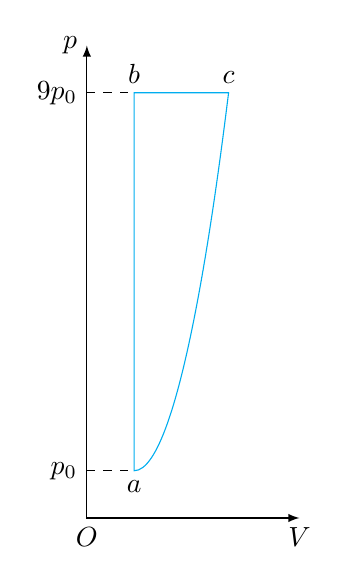
\begin{tikzpicture}[scale = 0.6]
            %画坐标轴
            \draw[latex-latex] (0, 10) -- (0, 0) -- (4.5, 0);
            \node[below] at (4.5,0) {$V$};
            \node[left ] at (0, 10) {$p$};
            \node[below] at (0, 0) {$O$};

            %画出虚线辅助线
            \draw[dashed] (0, 9) -- (1, 9);
            \draw[dashed] (0, 1) -- (1, 1);

            %画出p-V曲线
            \draw[cyan] (1,1) parabola (3,9) -- (1,9) -- (1,1) -- cycle;

            %标注出各个点
            \node[left ] at (0, 9) {$9p_0$};
            \node[left ] at (0, 1) {$p_0$};
            \node[below] at (1, 1) {$a$};
            \node[above] at (1, 9) {$b$};
            \node[above] at (3, 9) {$c$};
        \end{tikzpicture}
    \end{center}
\end{question}
\begin{solution}
    (1)对于 $a \to b$ 的等体过程,有$\frac{T_b}{p_b} = \dfrac{T_a}{p_a}$,则
    $$
        Q_{ab} = C_{V,\mathrm{m}}(T_b - T_a) = \frac{3}{2}R(9T_0 - T_0) = 12RT_0
    $$
    对于 $b \to c$ 的等压过程,有 $V_c = 3V_0$,$T_c = \dfrac{V_c}{V_b}T_b = 27T_0$,则
    $$
        Q_{bc} = C_{p,\mathrm{m}}(T_c - T_b) = \frac{5}{2}R(27T_0 - 9T_0) = 45RT_0
    $$
    对于 $c \to a$ 的多方过程,有$pV^{-2} = C$,多方指数为 $n=-2$,而多方过程的热容为
    $$
        C_{n,m} = C_{V,\mathrm{m}} \cdot \frac{\gamma - n}{1 - n} = \frac{11}{6}R
    $$
    于是得到
    $$
        Q_{ca} = C_{n,m}(T_a - T_c) = -47.7RT_0
    $$
    (2)这一循环的效率为
    $$
        \eta
        = \frac{|Q_{ab} + Q_{bc}| - |Q_{ca}|}{|Q_{ab} + Q_{bc}|}
        = \frac{12+45-47.7}{12+45}
        = 16.4\%
    $$
\end{solution}

\begin{question}{题目4.7.1}
    将热机与热泵组合在一起的暖气设备称为动力暧气设备,其中带动热泵的动力由热机燃烧燃料对外界做的功来提供. 热泵从天然蓄水池或从地下水取出热量,向温度较高的暖气系统的水供热同时,暖气系统的水又作为热机的冷却水. 若燃烧 $1 \,\si{kg}$ 燃料,锅炉能获得的热量为 $H$,锅炉、地下水、暖气系统的水的温度分别为 $210 \,\si{^\circ C}$,$15 \,\si{^\circ C}$,$60 \,\si{^\circ C}$. 设热机及热泵均是可逆卡诺机. 试问每燃烧 $1 \,\si{kg}$ 燃料,暖气系统所获得热量的理想数值(不计各种实际损)是多少?
\end{question}
\begin{solution}
    卡诺热机工作在锅炉和暖气系统之间,它先从锅炉获取热量 $H$,再做功 $W$ 驱动热泵,最后向暖气系统排放废热 $Q_1 = H - W$;而热泵工作于地下水和暖气系统之间,它被热机输出的功 $W$ 所驱动,从低温的地下水取热 $Q_2$ 并向暖气系统供热.

    热机工作在锅炉和暖气系统之间,根据卡诺热机效率 $\eta_\text{热}$ 的定义
    $$
        \eta_\text{热} = \frac{W}{H} = 1 - \frac{T_3}{T_1}
    $$
    导出热机用于驱动热泵的功 $W$
    $$
        W = \left(1-\frac{T_3}{T_1}\right) H
    $$
    热机做功后会继续向暖气排放废热
    $$
        Q_1 = H-W
        = H - \left(1 - \frac{T_3}{T_1} \right) H
        = \frac{T_3}{T_1}H
        \approx 0.69H
    $$
    热泵由热机所驱动,且热泵工作在地下水 $T_2$ 和暖气系统 $T_3$ 之间,那么根据热泵供热系数 $\varepsilon$ 的定义
    $$
        \varepsilon = \frac{Q}{W} = \frac{T_3}{T_3 - T_2}
    $$
    可以得到热泵从地下水取热 $Q_2$
    $$
        Q_2 = \frac{T_3}{T_3 - T_2} W
        = \left(\frac{T_3}{T_3 - T_2}\right) \left(1 - \frac{T_3}{T_1}\right) H
        \approx 2.30H
    $$
    最终暖气得到的热量 $Q_\text{暖气}$ 为热机排放的废热 $Q_1$ 和热泵从地下水抽取的热量 $Q_2$ 之和
    $$
        Q_\text{暖气} = Q_1 + Q_2
        = \frac{T_3}{T_1}H + \left(\frac{T_3}{T_3 - T_2}\right) \left(1 - \frac{T_3}{T_1}\right) H
        \approx 3.00H
    $$
    由此可见暖气最终得到的热量 $Q_\text{暖气}$ 约为锅炉燃烧产热 $H$ 的 3 倍.
\end{solution}